


\tikzset{every picture/.style={line width=0.75pt}} %set default line width to 0.75pt        

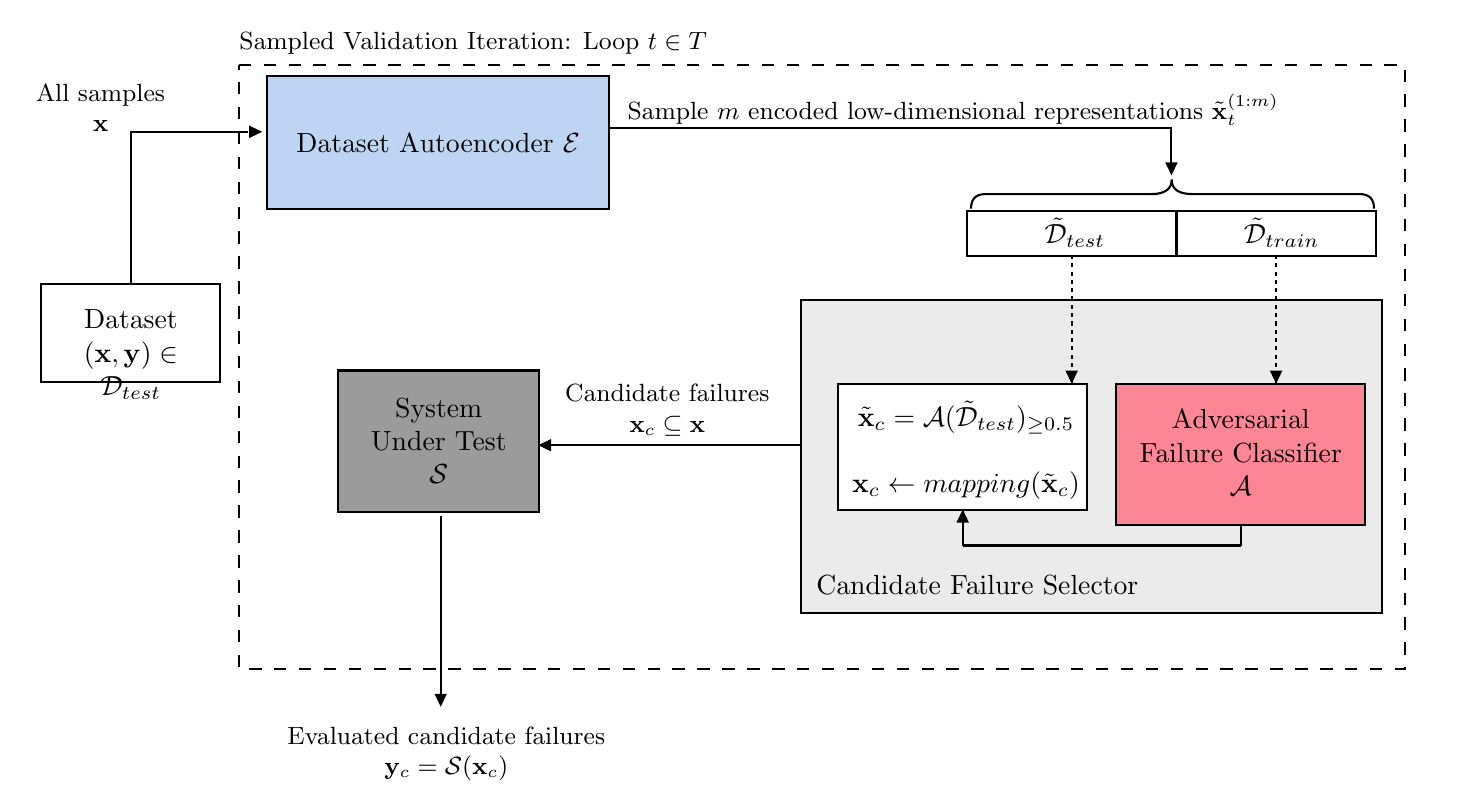
\begin{tikzpicture}[x=0.75pt,y=0.75pt,yscale=-1,xscale=1]
%uncomment if require: \path (0,399); %set diagram left start at 0, and has height of 399

%Shape: Rectangle [id:dp3416440849450273] 
\draw  [dash pattern={on 4.5pt off 4.5pt}][line width=0.75]  (91.17,38) -- (653.17,38) -- (653.17,329) -- (91.17,329) -- cycle ;
%Straight Lines [id:da6207923302069309] 
\draw    (39.17,144) -- (39.17,70) -- (95.5,70) ;
\draw [shift={(102.5,70)}, rotate = 180] [fill={rgb, 255:red, 0; green, 0; blue, 0 }  ][line width=0.08]  [draw opacity=0] (6.25,-3) -- (0,0) -- (6.25,3) -- cycle    ;
%Straight Lines [id:da40087733759777344] 
\draw    (257.17,68) -- (540.57,68) -- (540.57,88) ;
\draw [shift={(540.57,91)}, rotate = 270] [fill={rgb, 255:red, 0; green, 0; blue, 0 }  ][line width=0.08]  [draw opacity=0] (6.25,-3) -- (0,0) -- (6.25,3) -- cycle    ;
%Shape: Brace [id:dp16419611390886946] 
\draw   (638.17,107) .. controls (638.17,102.33) and (635.84,100) .. (631.17,100) -- (550.68,100) .. controls (544.01,100) and (540.68,97.67) .. (540.68,93) .. controls (540.68,97.67) and (537.35,100) .. (530.68,100)(533.68,100) -- (451,100) .. controls (446.33,100) and (444,102.33) .. (444,107) ;
%Straight Lines [id:da03991771123197685] 
\draw    (380.5,221) -- (235.5,221) ;
\draw [shift={(235.5,221)}, rotate = 360] [fill={rgb, 255:red, 0; green, 0; blue, 0 }  ][line width=0.08]  [draw opacity=0] (6.25,-3) -- (0,0) -- (6.25,3) -- cycle    ;
%Straight Lines [id:da4068130382497208] 
\draw    (188.5,255) -- (188.5,344) ;
\draw [shift={(188.5,347)}, rotate = 270] [fill={rgb, 255:red, 0; green, 0; blue, 0 }  ][line width=0.08]  [draw opacity=0] (6.25,-3) -- (0,0) -- (6.25,3) -- cycle    ;

% Text Node
\draw  [fill={rgb, 255:red, 189; green, 213; blue, 242 }  ,fill opacity=1 ]  (104.75,43.17) -- (269.75,43.17) -- (269.75,107.17) -- (104.75,107.17) -- cycle  ;
\draw (187.25,75.17) node   [align=left] {\begin{minipage}[lt]{109.32564pt}\setlength\topsep{0pt}
\begin{center}
Dataset Autoencoder $\displaystyle \mathcal{E}$
\end{center}

\end{minipage}};
% Text Node
\draw  [fill={rgb, 255:red, 155; green, 155; blue, 155 }  ,fill opacity=1 ]  (139.06,185) -- (236.06,185) -- (236.06,253) -- (139.06,253) -- cycle  ;
\draw (187.56,219) node   [align=left] {\begin{minipage}[lt]{63.197500000000005pt}\setlength\topsep{0pt}
\begin{center}
System\\Under Test\\$\displaystyle \mathcal{S}$
\end{center}

\end{minipage}};
% Text Node
\draw (90,20.33) node [anchor=north west][inner sep=0.75pt]  [font=\small] [align=left] {Sampled Validation Iteration: Loop $\displaystyle t \in T$};
% Text Node
\draw  [fill={rgb, 255:red, 255; green, 255; blue, 255 }  ,fill opacity=1 ]  (-4,143.33) -- (82,143.33) -- (82,190.33) -- (-4,190.33) -- cycle  ;
\draw (2,154.33) node [anchor=north west][inner sep=0.75pt]   [align=left] {\begin{minipage}[lt]{53.541216pt}\setlength\topsep{0pt}
\begin{center}
Dataset \\$\displaystyle (\mathbf{x}, \mathbf{y}) \in \mathcal{D}_\text{test}$
\end{center}

\end{minipage}};
% Text Node
\draw (-10,45.33) node [anchor=north west][inner sep=0.75pt]  [font=\small] [align=left] {\begin{minipage}[lt]{49.655912pt}\setlength\topsep{0pt}
\begin{center}
All samples\\$\displaystyle \mathbf{x}$
\end{center}

\end{minipage}};
% Text Node
\draw (277,50.33) node [anchor=north west][inner sep=0.75pt]  [font=\small] [align=left] {Sample $m$ encoded low-dimensional representations $\displaystyle \tilde{\mathbf{x}}_{t}^{(1:m)}$};
% Text Node
\draw  [fill={rgb, 255:red, 255; green, 255; blue, 255 }  ,fill opacity=1 ]  (442,108) -- (543,108) -- (543,130) -- (442,130) -- cycle  ;
\draw (478,110) node [anchor=north west][inner sep=0.75pt]   [align=left] {$\displaystyle \tilde{\mathcal{D}}_{\text{test}}$};
% Text Node
\draw  [fill={rgb, 255:red, 235; green, 235; blue, 235 }  ,fill opacity=1 ]  (362,151) -- (642,151) -- (642,302) -- (362,302) -- cycle  ;
\draw (368,282) node [anchor=north west][inner sep=0.75pt]   [align=left] {Candidate Failure Selector};
% Text Node
\draw  [fill={rgb, 255:red, 252; green, 134; blue, 148 }  ,fill opacity=1 ]  (514,191.33) -- (634,191.33) -- (634,259.33) -- (514,259.33) -- cycle  ;
\draw (520,202.33) node [anchor=north west][inner sep=0.75pt]   [align=left] {\begin{minipage}[lt]{78.6726pt}\setlength\topsep{0pt}
\begin{center}
Adversarial\\Failure Classifier\\$\displaystyle \mathcal{A}$
\end{center}

\end{minipage}};
% Text Node
% \draw  [fill={rgb, 255:red, 255; green, 255; blue, 255 }  ,fill opacity=1 ]  (419.5, 222) circle [x radius= 26.54, y radius= 26.54]   ;
\draw  [fill={rgb, 255:red, 255; green, 255; blue, 255 }  ,fill opacity=1 ]  (380,191.33) -- (500,191.33) -- (500,252) -- (380,252) -- cycle  ;
\draw (385,198) node [anchor=north west][inner sep=0.75pt]   [align=left] {\begin{minipage}[lt]{82.6726pt}\setlength\topsep{0pt}
\begin{center}
$\tilde{\mathbf{x}}_c = \mathcal{A}(\tilde{\mathcal{D}}_\text{test})_{\ge 0.5}$\\
\phantom{}\\
$\mathbf{x}_c \leftarrow \operatorname{mapping}(\tilde{\mathbf{x}}_c)$
\end{center}
\end{minipage}};

% Text Node
\draw (245,190.33) node [anchor=north west][inner sep=0.75pt]  [font=\small] [align=left] {\begin{minipage}[lt]{76.7176pt}\setlength\topsep{0pt}
\begin{center}
Candidate failures\\$\displaystyle \mathbf{x}_{c} \subseteq \mathbf{x}$
\end{center}

\end{minipage}};
% Text Node
\draw (111,355.33) node [anchor=north west][inner sep=0.75pt]  [font=\small] [align=left] {\begin{minipage}[lt]{118.05956pt}\setlength\topsep{0pt}
\begin{center}
Evaluated candidate failures\\$\displaystyle \mathbf{y}_{c} =\mathcal{S}(\mathbf{x}_{c})$
\end{center}

\end{minipage}};
% Text Node
\draw  [fill={rgb, 255:red, 255; green, 255; blue, 255 }  ,fill opacity=1 ]  (543,108) -- (639,108) -- (639,130) -- (543,130) -- cycle  ;
\draw (574,110) node [anchor=north west][inner sep=0.75pt]   [align=left] {$\displaystyle \tilde{\mathcal{D}}_{\text{train}} \ \ \ \ \ \ \ \ \ \ \ \ $};

%Straight Lines [id:D_train -> Adversary] 
\draw  [dash pattern={on 1.5pt off 1.5pt}][line width=0.75]  (591,191.33) -- (591,130) ;
\draw [shift={(591,191.33)}, rotate = 270] [fill={rgb, 255:red, 0; green, 0; blue, 0 }  ][line width=0.08]  [draw opacity=0] (6.25,-3) -- (0,0) -- (6.25,3) -- cycle    ;

%Straight Lines [id:D_test -> Candidate selector] 
\draw  [dash pattern={on 1.5pt off 1.5pt}][line width=0.75]  (492.5,191.33) -- (492.5,130) ;
\draw [shift={(492.5,191.33)}, rotate = 270] [fill={rgb, 255:red, 0; green, 0; blue, 0 }  ][line width=0.08]  [draw opacity=0] (6.25,-3) -- (0,0) -- (6.25,3) -- cycle    ;

%Straight Lines [id:Adversary -> Candidate selector] 
\draw  (574,259.33) -- (574,269.33) ;
\draw  (574,269.33) -- (440,269.33) ;
\draw  (440,269.33) -- (440,252) ;
\draw [shift={(440,252)}, rotate = 90] [fill={rgb, 255:red, 0; green, 0; blue, 0 }  ][line width=0.08]  [draw opacity=0] (6.25,-3) -- (0,0) -- (6.25,3) -- cycle    ;


\end{tikzpicture}
